\section{The Client, the Customer and Other Stakeholders}

\subsection{The Client}

 % Client
	\textbf{Dr Hugh \textsc{Osborne}}\\
	Senior Lecturer\\
	University Of Huddersfield\\
	h.r.osborne@hud.ac.uk

\subsection{The Customer}

The intended customer of the product are users of smartphone and tablets whom are looking to solve all those unsolvable Cryptic Crosswords. The applications will be deployed on the app market for the three listed mobile operating systems which means that the app will be available to anyone who has a compatible device with the required software. The physical deployment of the application is out of the project scope so a price for the deployment will not be discussed.

\subsection{Other Stakeholders}

For the purpose of the project the other stakeholders are as follows:

 % Supervisor
      \emph{Project Supervisor}\\
      \textbf{Dr. Gary \textsc{Allen}} \\
      Senior Lecturer \\
      University Of Huddersfield \\
      g.allen@hud.ac.uk 

  % Examiner
      \emph{Project Examiner:} \\ 
      \textbf{Sotirios \textsc{Batsakis}}\\
      University Of Huddersfield\\
      s.batsakis-STA@unimail.hud.ac.uk

  % Moderator
      \emph{Internal Moderator}\\
      \textbf{Collin \textsc{Venters}} \\
      Senior Lecturer \\
      University Of Huddersfield \\
      c.venters@hud.ac.uk

\subsection{The Hands-On Users of the Product}

To determine the users of the product it was decided yo carry out a survey in
order to identify the potential users that actually will be using the product.

The following questions were asked:

\begin{itemize}
    \item Do you play Cryptic Crosswords?
    \item How Often do you play?
    \item Where do you play?
    \item Do you often finish them?
    \item If no to the previous question, what reason don't you finish them?
    \item What is your age group?
    \item When do you play Cryptic Crosswords?
    \item What gender are you?
    \item What is the Highest qualification you have?
    \item What platform is your mobile phone on?
\end{itemize}

The survey was conducted between (date) and (date). It was distributed across
the Department of Computing And Engineering at the University Of Huddersfield,
Facebook and Twitter. The results of this survey are shown in Figure
~\ref{fig:survey_results}


\begin{figure}[here]
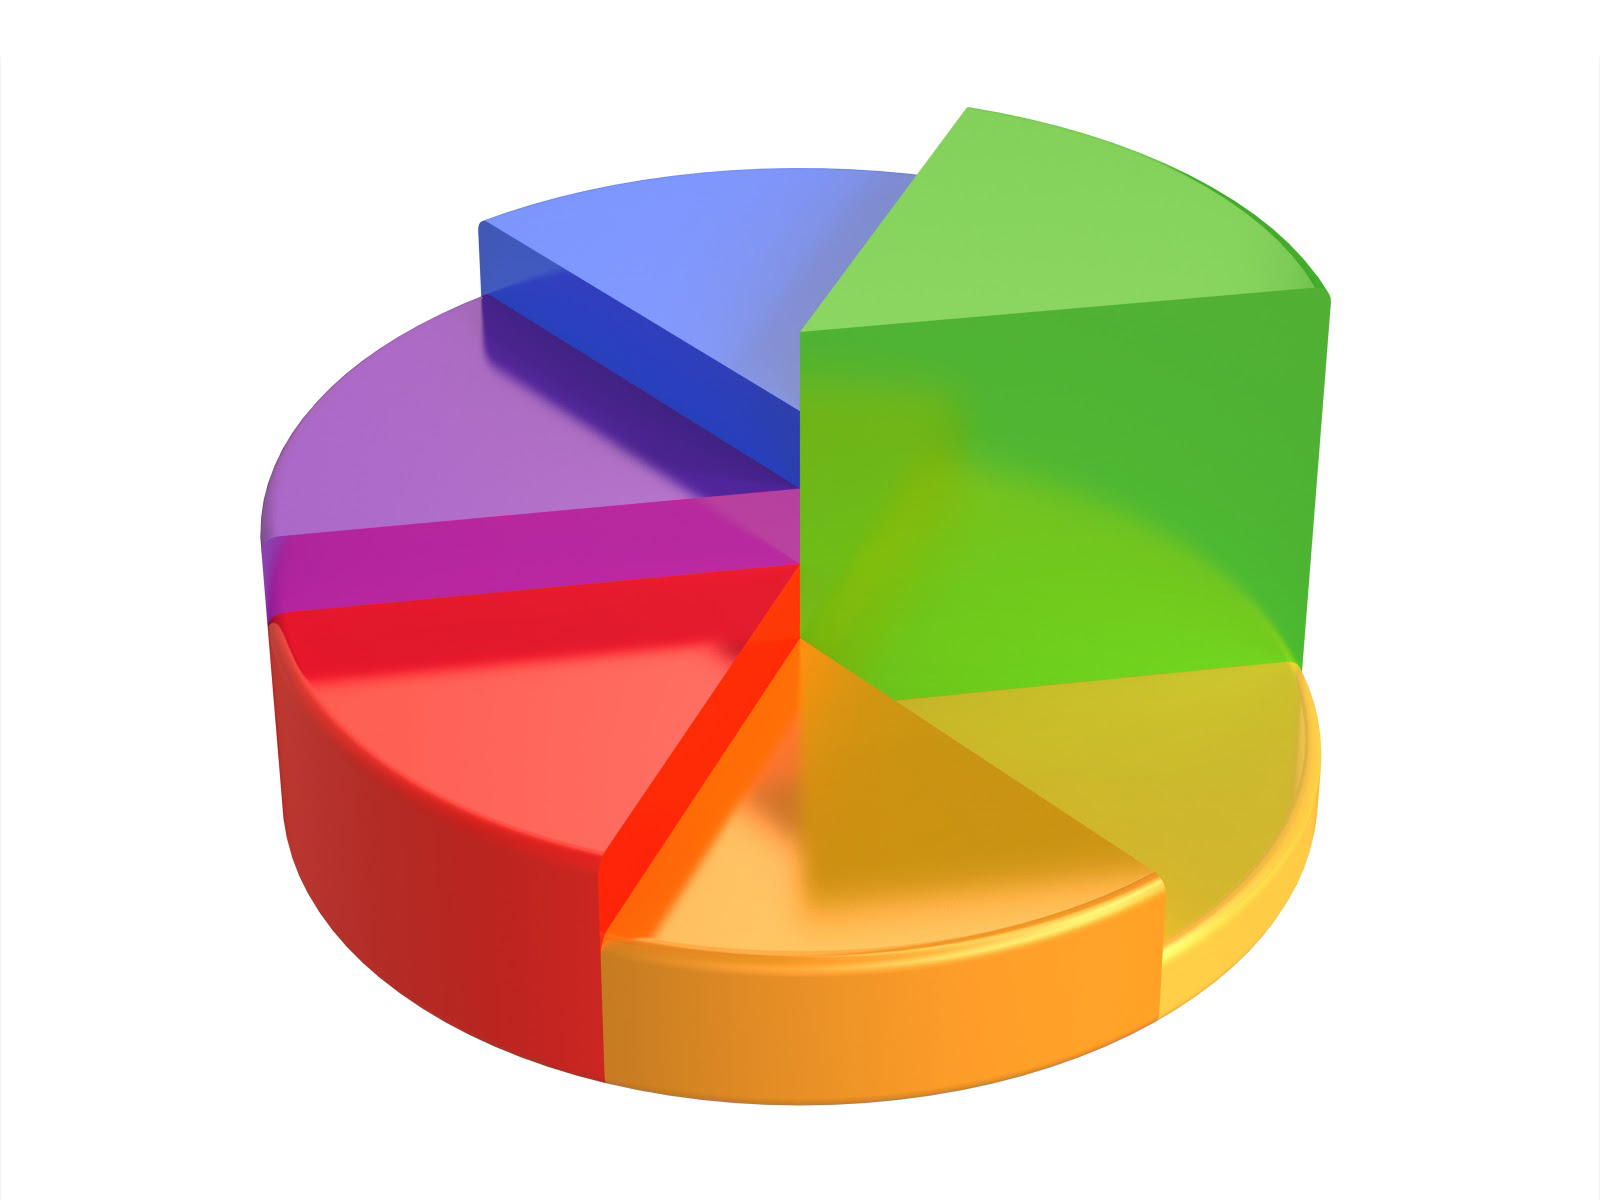
\includegraphics[width=0.9\textwidth]{requirements/project_drivers/survey_results.png}
\caption{Cryptic Crosswords Survey Results}
\label{fig:survey_results}
\end{figure}

From these results it can be deduced that .....